\documentclass{article}
\usepackage{tabularx}
\usepackage{setspace}
\usepackage{graphicx}
\usepackage{amsmath}
\usepackage{xcolor}
\usepackage{amssymb}
\usepackage[margin=1in]{geometry}
\usepackage{tikz}
\usetikzlibrary{automata}
\usetikzlibrary{positioning}
\usetikzlibrary{arrows}
\tikzset{	node distance=2.5cm, 
	every state/.style={ 
		semithick,
		fill=gray!10},
	initial text={},     
	double distance=2pt, 
	every edge/.style={  
		draw,
		->, %>=stealth’,     
		auto,
		semithick}
}
\let\epsilon\varepsilon
\usepackage{xepersian}
\settextfont{X Yas}
% Fixture for Xepersian 23 bug of setting persian math digit fonts
\ExplSyntaxOn \cs_set_eq:NN \etex_iffontchar:D \tex_iffontchar:D \ExplSyntaxOff
\setmathdigitfont{X Yas}
\onehalfspacing
\renewcommand{\labelenumii}{\alph{enumii})}


\begin{document}
	\begin{center}
		\Huge
		مبانی نظریه محاسبه
	\end{center}
	\Large
	\begin{tabularx}{\linewidth}{>{\raggedleft\arraybackslash}X>{\raggedright\arraybackslash}X}
		پاسخ کوییز  دوم
		&
		نمره کل: 25
	\end{tabularx}
	\rule{\textwidth}{1pt}
	\begin{enumerate}
		\item 
		
		\textcolor{cyan}{
			(7 نمره)
		}
	
		 
	
	
	\begin{figure}[h]
		\centering
		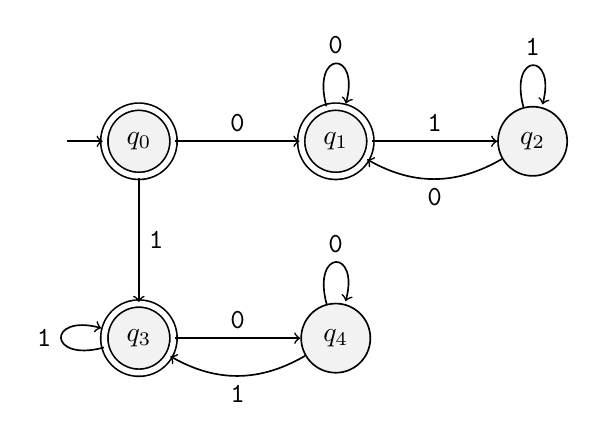
\begin{tikzpicture}
			\node[state, accepting, initial] (q0) {$q_0$};
			\node[state, accepting, right of=q0] (q1) {$q_1$};
			\node[state,  right of=q1] (q2) {$q_2$};
			\node[state, , accepting, below of=q0] (q3) {$q_3$};
			\node[state,  right of=q3] (q4) {$q_4$};
			\draw (q1) edge[loop above] node {\tt 0} (q1);
			\draw (q2) edge[loop above] node {\tt 1} (q2);
			\draw (q3) edge[loop left] node {\tt 1} (q3);
			\draw (q4) edge[loop above] node {\tt 0} (q4);
			\draw (q0) edge node {\tt 0} (q1);
			\draw (q1) edge node {\tt 1} (q2);
			\draw (q0) edge node {\tt 1} (q3);
			\draw (q3) edge node {\tt 0} (q4);
			\draw (q2) edge[bend left] node {\tt 0} (q1);
			\draw (q4) edge[bend left] node {\tt 1} (q3);
		\end{tikzpicture}
	
	\end{figure}
		
		
		\item 
		
		\textcolor{cyan}{
			(4 نمره)
		}
	
	
		
		
		\begin{figure}[h]
			\centering
			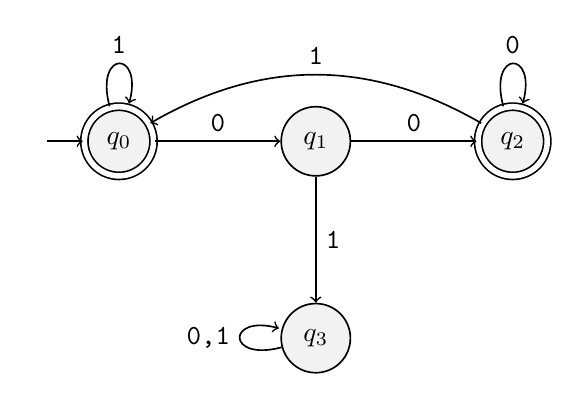
\begin{tikzpicture}
				\node[state, accepting,initial] (q0) {$q_0$};
				\node[state, right of=q0] (q1) {$q_1$};
				\node[state,  accepting, right of=q1] (q2) {$q_2$};
				\node[state, below of=q1] (q3) {$q_3$};
				\draw (q0) edge node {\tt 0} (q1);
				\draw (q1) edge node {\tt 0} (q2);
				\draw (q1) edge node {\tt 1} (q3);
				\draw (q0) edge[loop above] node {\tt 1} (q0);
				\draw (q2) edge[loop above] node {\tt 0} (q2);
				\draw (q3) edge[loop left] node {\tt 0,1} (q3);
				\draw (q2) edge[bend right] node [above] {\tt 1} (q0);
			\end{tikzpicture}
			
		\end{figure}
		
		
		
		
		
		\item 
		
		\textcolor{cyan}{
			(5 نمره)
		}
		
		
		
		
		\begin{figure}[h]
			\centering
			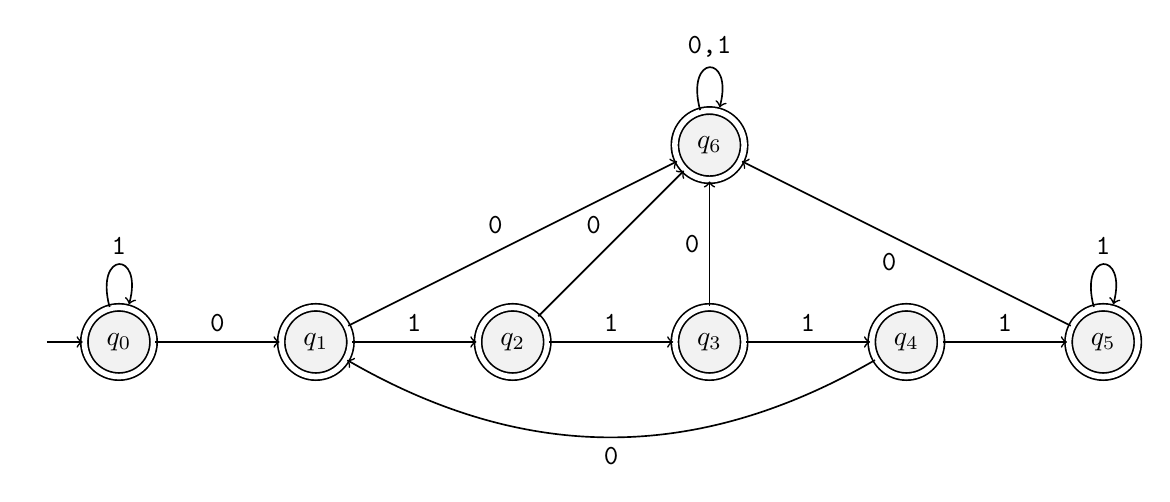
\begin{tikzpicture}
				\node[state, accepting,initial] (q0) {$q_0$};
				\node[state, accepting, right of=q0] (q1) {$q_1$};
				\node[state, accepting, right of=q1] (q2) {$q_2$};
				\node[state, accepting, right of=q2] (q3) {$q_3$};
				\node[state, accepting, right of=q3] (q4) {$q_4$};
				\node[state, accepting, right of=q4] (q5) {$q_5$};
				\node[state, accepting, above of=q3] (q6) {$q_6$};
				\draw (q0) edge[loop above] node {\tt 1} (q0);
				\draw (q5) edge[loop above] node {\tt 1} (q5);
				\draw (q6) edge[loop above] node {\tt 0,1} (q6);
				\draw (q0) edge node {\tt 0} (q1);
				\draw (q1) edge node {\tt 1} (q2);
				\draw (q2) edge node {\tt 1} (q3);
				\draw (q3) edge node {\tt 1} (q4);
				\draw (q4) edge node {\tt 1} (q5);
				\draw (q5) edge node {\tt 0} (q6);
				\draw (q1) edge node {\tt 0} (q6);
				\draw (q2) edge node {\tt 0} (q6);
				\draw (q3) edge node {\tt 0} (q6);
				\draw (q4) edge[bend left] node {\tt 0} (q1);
			\end{tikzpicture}
			
		\end{figure}
		
		
		
		\item 
		
		\textcolor{cyan}{
			(9 نمره)
		}
		
		
		
		
		\begin{figure}[h]
			\centering
			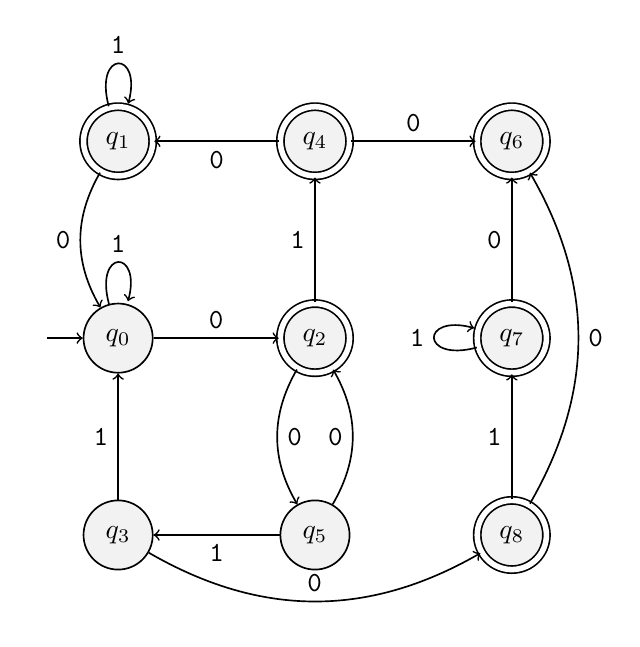
\begin{tikzpicture}
				\node[state, initial] (q0) {$q_0$};
				\node[state, accepting, above of = q0] (q1) {$q_1$};
				\node[state, accepting, right of = q0] (q2) {$q_2$};
				\node[state, below of =q0] (q3) {$q_3$};
				\node[state, accepting, above of = q2] (q4) {$q_4$};
				\node[state, below of = q2] (q5) {$q_5$};
				\node[state, accepting, right of = q4] (q6) {$q_6$};
				\node[state, accepting, right of = q2] (q7) {$q_7$};
				\node[state, accepting, below of = q7] (q8) {$q_8$};
				\draw (q0) edge[loop above] node {\tt 1} (q0);
				\draw (q1) edge[loop above] node {\tt 1} (q1);
				\draw (q7) edge[loop left] node {\tt 1} (q7);
				\draw (q0) edge node {\tt 0} (q2);
				\draw (q2) edge node {\tt 1} (q4);
				\draw (q2) edge[bend right] node {\tt 0} (q5);
				\draw (q1) edge[bend right] node [left]{\tt 0} (q0);
				\draw (q5) edge[bend right] node {\tt 0} (q2);
				\draw (q3) edge node {\tt 1} (q0);
				\draw (q5) edge node {\tt 1} (q3);
				\draw (q4) edge node {\tt 0} (q1);
				\draw (q3) edge[bend right] node {\tt 0} (q8);
				\draw (q4) edge node {\tt 0} (q6);
				\draw (q7) edge node {\tt 0} (q6);
				\draw (q8) edge node {\tt 1} (q7);
				\draw (q8) edge[bend right] node[right] {\tt 0} (q6);
			\end{tikzpicture}
			
		\end{figure}
		
		
	\end{enumerate}
\end{document}